\RequirePackage{xcolor}
\documentclass[a4]{sciposter}
\usepackage{multicol,subfig,amsmath} % columnas, figuras, ecuaciones
\usepackage{graphicx,url,hyperref,doi}
\hypersetup{hidelinks} 
\usepackage[spanish]{babel}   
\usepackage[utf8]{inputenc}
\usepackage[sort&compress,numbers]{natbib}
\usepackage[font=small,labelfont=bf]{caption}

\usepackage{tikz} % diagramas
\tikzstyle{elem} = [draw, rectangle, thick, minimum height=2em, minimum width=2em]
\tikzstyle{line} = [draw, thick, -stealth, shorten >=1pt]

\setlength{\parskip}{3pt} % espacio entre parrafos
\renewcommand{\arraystretch}{1.5} % altura de renglones de cuadros

\title{Nombre de tu proyecto}
\author{Alumno de Verano y Elisa Schaeffer}
\institute {Posgrado en Ingeniería de Sistemas}
\email{alumno.verano@instituto.edu.mx}

\leftlogo[1]{uanl.png} 
\rightlogo[1]{fime.png}

\begin{document}

\conference{Verano Científico 2021 ---
  Facultad de Ingeniería Mecánica y Eléctrica ---
  Universidad Autónoma de Nuevo León}

\maketitle
\begin{abstract}
En el resumen describes brevemente todo el proyecto, desde qué se
trata hasta qué lograste hacer.
\end{abstract}

\begin{multicols}{2} 

\section{Introducción}

De qué se trata el proyecto. Hipótesis y objetivos. Motivación, justificación.

\section{Antecedentes}

Conceptos y notación indispensables para que tus lectores puedan
entender el resto del trabajo. Citamos al libros de texto como el de
\citet{ai}.

\section{Estado de arte}

Qué han hecho los demás sobre este tema (citar a publicaciones
científicas, de preferencia publicadas en revistas que tengan DOI y
que por lo menos algunos sean de los últimos cinco años. Aquí se
suelen citar artículos como por ejemplo el trabajo de \citet{elisa} o
algo que se haya presentado en un congreso como \citet{ar}. A veces es
necesario definir algo matemático como por ejemplo
\begin{equation}
    f(x) = \sum_{i = 0}^\infty \sin(i x)
    \label{suma}
\end{equation}
para comunicar mejor lo que pasa.

Si una ecuación depende de otra, conviene mencionarlo de manera
explícita. Por ejemplo se puede poner $g(x) = \sqrt{f(x)}$, donde
$f(x)$ proviene de la ecuación \eqref{suma}.

Área de oportunidad: qué exactamente este trabajo contribuirá encima
de lo que ya existe.  {\textquestiondown}Qué tiene de
diferente/original/impacto?

\section{Solución propuesta}

Metodología, herramientas (qué en sí haces, cómo lo haces, con qué lo
haces).  La implementación se hizo en Python 3.9 \citep{python} y los
componentes se interconectan como muestra el diagrama de la figura
\ref{diag}.

\begin{figure}
\captionsetup{type=figure} % por culpa de sciposter
\setcounter{figure}{0} % por culpa de sciposter
\begin{center}
    \begin{tikzpicture}[]
      \matrix[row sep=0.5cm]{
      \node[elem] (n1) {Una cosa}; & & \node[elem] (n2) {Otra cosa}; \\
      & \node[elem] (n3) {Nueva cosa}; & \\
      };
     \draw [line] (n1) -- (n2);
     \draw [line] (n1) -- (n3);
     \draw [line] (n2) -- (n3);
    \end{tikzpicture}
\end{center}
\caption{Hay que explicar qué quieren decir los elementos de la figura.}
\label{diag}
\end{figure}

\section{Experimentos}

Diseño, reportaje y análisis de los resultados de los
experimentos. Por lo general se incluyen figuras como la figura
\ref{curvas}.

\begin{figure}
% por culpa de sciposter, hay que ajustar numeracion manualmente  
\setcounter{figure}{1} 
\captionsetup{type=figure} % por culpa de sciposter
\begin{center}
   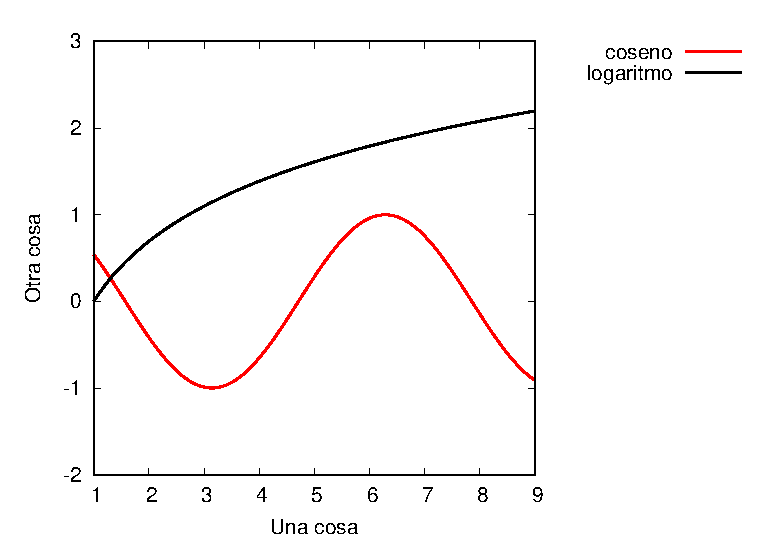
\includegraphics[width=0.5\textwidth]{curvas.eps}
   \end{center}
    \caption{Hay que explicar qué quieren decir los elementos de la figura.}
    \label{curvas}
\end{figure}

Además es muy común incluir cuadros de datos, como por ejemplo el cuadro \ref{data}.

\begin{table}
\setcounter{table}{0} % por culpa de sciposter
\captionsetup{type=table} % por culpa de sciposter
\caption{Aquí explicas cómo interpreta el cuadro.}
\label{data}
\begin{center}
\scalebox{0.9}{\begin{tabular}{|r|c|l|}
    \hline
         \multicolumn{1}{|c|}{\rotatebox{90}{\bf Valor}}
         & \multicolumn{1}{|c|}{\rotatebox{90}{\bf Parámetro}}
         & \multicolumn{1}{|c|}{\rotatebox{90}{\bf Descripción\phantom{m}}} \\
         \hline
         0.23 & $x$ & algo \\
         \hline
         2.34 & $y$ & demo \\
        \hline
    \end{tabular}}
\end{center}
\end{table}

\section{Conclusiones}

Qué se logró hacer; qué posibilidad de trabajo a futuro se tiene para
este trabajo.

\paragraph{Agradecimientos}

{\small Mencionar organismos que otorgaron beca como Delfín o
  PROVERICYT. Agradecer a las demás personas que \underline{no son
    autores} quienes ayudaron en algo. Además estaría padre mencionar
  que el póster se preparó con \url{https://www.overleaf.com/}.}

\end{multicols}

\bibliography{poster}
\bibliographystyle{plainnat}

\end{document}
